\documentclass[20 pt, a0paper, portrait]{tikzposter}
\usepackage[utf8]{inputenc}
\usepackage{amsmath}
\usepackage{amssymb}
\usepackage{algorithm,algorithmic}
\usepackage{pgfplots}

% Algorithmic modifications
\makeatletter
\newcommand{\ALOOP}[1]{\ALC@it\algorithmicloop\ #1 ~\algorithmicdo\begin{ALC@loop}}
\newcommand{\ENDALOOP}{\end{ALC@loop}\ALC@it\algorithmicendloop}
\renewcommand{\algorithmicloop}{\textbf{parfor}}
\makeatother

\geometry{paperwidth=24in,paperheight=36in}
\makeatletter
\setlength{\TP@visibletextwidth}{\textwidth-2\TP@innermargin}
\setlength{\TP@visibletextheight}{\textheight-2\TP@innermargin}
\makeatother

\title{Fourth Order Modified Laguerre's Method}
\author{Thomas R. Cameron}
\date{\today}
\institute{Davidson College}
 
\usepackage{blindtext}
\usepackage{comment}

\usetheme{Autum}
 
\begin{document}
 
\maketitle

%%%%%%%%%%%%%%%%%%%%%%%%%%%%%%%%%%%%%%%%
%								Abstract						%
%%%%%%%%%%%%%%%%%%%%%%%%%%%%%%%%%%%%%%%%
\block{Abstract}
{
We present a novel modification of Laguerre's method that results in a method for the concurrent approximation of all roots of a univariate polynomial. Our method has strong virtues including fourth-order convergence that is observed in practice and belonging to the class of embarrassingly parallel algorithms. A Fortran 90 implementation of our algorithm is available online and comparisons with several other software are provided to show the effectiveness of our approach.
}

%%%%%%%%%%%%%%%%%%%%%%%%%%%%%%%%%%%%%%%%
%					The Algorithm and Examples					%
%%%%%%%%%%%%%%%%%%%%%%%%%%%%%%%%%%%%%%%%
\begin{columns}
	\column{0.6}
	\block{The Algorithm}
	{
		Let $p(\lambda)=a_{0}+a_{1}\lambda+\cdots+a_{m}\lambda^{m}$ be a polynomial with $a_{0}a_{m}\neq 0$ and denote by $(z_{1},\ldots,z_{m})$ the current approximations to the roots $r_{1},\ldots,r_{m}$ of $p(\lambda)$. The $j$th approximation is updated via
		\begin{equation}
		\hat{z}_{j}=z_{j}-\frac{m}{G_{j}\pm\sqrt{(m-1)(mH_{j}-G_{j}^{2})}},
		\end{equation}
		where 
		\begin{equation}
		G_{j}=\frac{p^{'}(z_{j})}{p(z_{j})}-\sum_{\substack{i=1\\i\neq j}}^{m}\frac{1}{(z_{j}-z_{i})}~\text{ and }~H_{j}=-\left(\frac{p^{'}(z_{j})}{p(z_{j})}\right)^{'}-\sum_{\substack{i=1\\i\neq j}}^{m}\frac{1}{(z_{j}-z_{i})^{2}}.
		\end{equation}
		On each iteration, $z_{j}$ is updated for $j=1,\ldots,m$, unless it was accepted on a previous iteration. In this sense, all roots of the polynomial are approximated concurrently, rather than sequentially.
		
	\textbf{Initial Estimates} In essence, we select complex numbers along circles of suitable radii. What constitues suitable radii is formalized in~\cite{Bini1996} and can be computed via the upper envelope of the convex hull of the set $\{(i,\log|a_{i}|),~i=0,1,\ldots,m\}$. We compute the convex hull via Andrew's Monotone Chain algorithm~\cite{Andrew1979}.
	
	\textbf{Backward Error} The backward error of an approximate root $\xi$ is given by
	\begin{equation}
	\eta(\xi)=\frac{|p(\xi)|}{\alpha(\xi)},
	\end{equation}
	where $\alpha(\xi) = \sum_{i=0}^{m}|e_{i}||\xi|^{i}$ and $e_{i}$ are arbitrary and represent tolerances against which perturbations will be measured. We accept a root approximation $\xi$ if $\eta(\xi)<\mu$, where $\mu$ is machine precision. 
	
	\textbf{Condition} The condition of a nonzero approximate root $\xi$ is given by
	\begin{equation}
	\kappa(\xi)=\frac{\alpha(\xi)}{|\xi||p^{'}(\xi)|}.
	\end{equation}
	If the root approximation $\xi$ is accepted, then we also return its condition. Thus, we are able to give the upper bound $\eta(\xi)\cdot\kappa(\xi)$ on the forward error in the root approximation $\xi$. 
	}
	
	\column{0.4}
	\block{Examples}
	{
	\textbf{Initial Estimates} Let
	\[
	p(\lambda)=1+3\cdot10^{3}\lambda+3\cdot10^{6}\lambda^{2}+1\cdot10^{9}\lambda^{9}+\lambda^{10}.
	\] 
	The initial estimates and exact roots of $p$ are below.
	\begin{tikzfigure}
	\centering
	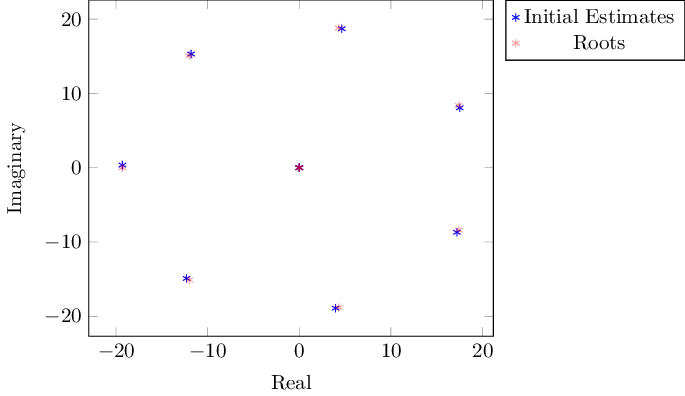
\includegraphics[scale=0.85]{../tests/figures/init_est_acc.png}
	\end{tikzfigure}
	
	\textbf{Convergence} Here we test the convergence of the roots of three polynomials. The first polynomial is $z^{5}-1$, the second is the degree $10$ Chebyshev polynomial, and the third is $z^{10}+\cdots+z+1$. The error is measured as the maximum relative forward error. For each polynomial, the error after each iteration is recorded in the table below.
	\vspace*{-2em}
	\begin{tikzfigure}
	\centering
	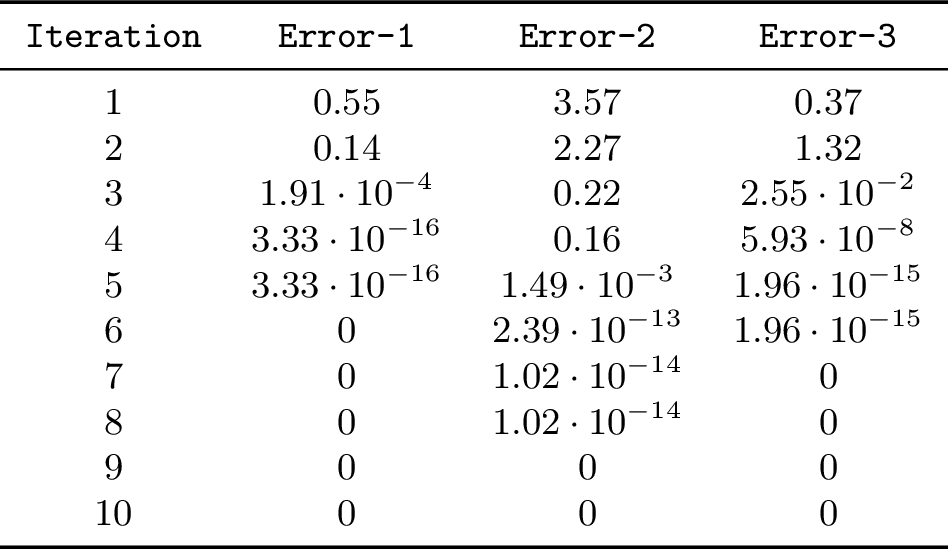
\includegraphics[scale=0.60]{../tests/figures/conv.png}
	\end{tikzfigure}
	}
 \end{columns}
 %%%%%%%%%%%%%%%%%%%%%%%%%%%%%%%%%%%%%%%%
%					Numerical Experiments						%
%%%%%%%%%%%%%%%%%%%%%%%%%%%%%%%%%%%%%%%%
 \begin{columns}
 	\column{0.6}
	\block{Numerical Experiments}
	{
	Comparisons betweeen FPML, Polzeros~\cite{Bini1996}, and the singleshift version of AMVW~\cite{Aurentz2015} are provided below.
	\begin{tikzfigure}
	\centering
	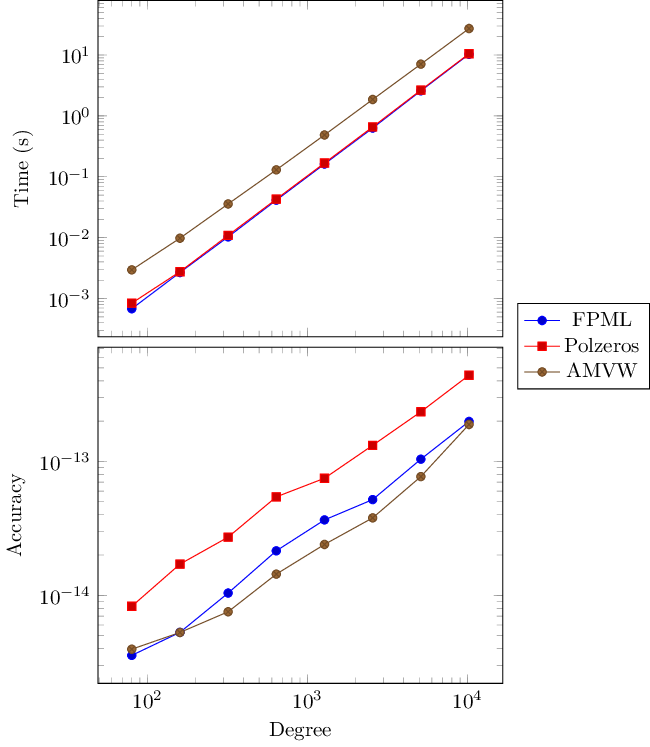
\includegraphics[scale=0.60]{../tests/figures/rand_poly.png}
	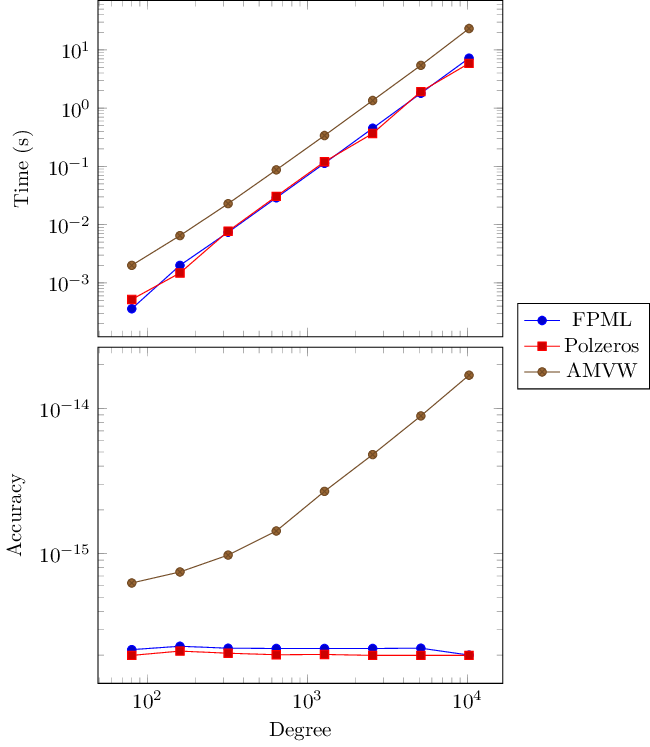
\includegraphics[scale=0.60]{../tests/figures/unity.png}
	\end{tikzfigure}
	}
	
	\column{0.4}
	\block{Conclusion}
	{
		\bibliographystyle{amsplain}
		\bibliography{Bibliography}
	}
 \end{columns}
 
\end{document}